% -*- coding: utf-8 -*-
\documentclass[aspectratio = 43]{beamer}
\usetheme{AnnArbor}
% set captions with numbers
\setbeamertemplate{caption}[numbered]


\usepackage{amsmath, nccmath}
\usepackage{booktabs}
\usepackage[utf8]{inputenc}
\usepackage[french]{babel}
\usepackage[T1]{fontenc}
\usepackage[backend=biber]{biblatex}
\addbibresource{biblio.bib}


\definecolor{halfgray}{gray}{0.8}

\usecolortheme{whale}
\setbeamercolor{frametitle}{parent=structure,bg=halfgray}

% Include other packages here, before hyperref.
\DeclareGraphicsExtensions{.pdf,.png,.jpg,.jpeg}
\graphicspath{{Figures/}} %Where the figures folder is located

%%%%%%%%%%%%%%%%%%%%%%%%%%%%%%%%%%%%%%%%%%%%%%%%%%
\usepackage{pgffor}
\usepackage{listings}
\usepackage[%font=bf,
skip=3pt]{caption}

\captionsetup[lstlisting]{font={tiny,tt}}
\setbeamerfont{caption}{size=\tiny}
%\setlength\abovecaptionskip{-1pt}
\usepackage{pythonhighlight}
\usepackage{xcolor}

\definecolor{codegreen}{rgb}{0,0.6,0}
\definecolor{codegray}{rgb}{0.5,0.5,0.5}
\definecolor{codepurple}{rgb}{0.58,0,0.82}
\definecolor{backcolour}{rgb}{0.95,0.95,0.92}

\lstdefinestyle{mystyle}{%
    backgroundcolor=\color{backcolour},
    commentstyle=\color{codegreen},
    keywordstyle=\color{magenta},
    numberstyle=\tiny\color{codegray},
    stringstyle=\color{codepurple},
    basicstyle=\ttfamily\footnotesize,
    breakatwhitespace=false,
    breaklines=true,
    captionpos=b,
    keepspaces=true,
    numbers=left,
    numbersep=1pt,
    showspaces=false,
    showstringspaces=false,
    showtabs=false,
    tabsize=2,
}

\lstset{style=mystyle}
%\usepackage{python}
%%%%%%%%%%%%%%%%%%%%%%%%%%%%%%%%%%%%%%%%%%%%%%%%%%

\title{Revue de Projet}
\subtitle{Classification et Comptage de contenants vides}
\author[]{\tiny Thomas CHECCHIN $-$ Dorian CHEVALERIAS $-$ Nicolas TO VAN
  TRANG $-$ Za{\"\i}d GHALI}
\institute[]{\textbf{T{\'e}l{\'e}com Physique Strasbourg}\\
  \textbf{SEW \-{} Usocome}}
\date{\tiny \today}


\begin{document}

%%%%--1--%%%%
\begin{frame}
  \begin{minipage}[t][0.2\textheight][t]{\textwidth}
    \centering
    
\includegraphics[scale=0.3,width=0.2\textwidth]{tps-logo.png}%
    \label{fig:tps_logo}
    \hspace*{4cm}
    
\includegraphics[scale=0.3,width=0.2\textwidth]{SEW_logo.jpg}%
    \label{fig:sew_logo}
  \end{minipage}
  \titlepage%
\end{frame}
%%%% --2--%%%%
\begin{frame}
  \frametitle{Plan}
  \tableofcontents
\end{frame}
%
% %%%% --3--%%%%
% \begin{itemize}
% \item Pr{\'e}sentation entreprise
% \item Etat actuel
% \end{itemize}

% -*- coding: utf-8 -*-
\section{Remise en contexte}
\subsection{Pr{\'e}sentation de l'entreprise}
\begin{frame}
  \frametitle{Pr{\'e}sentation de l'entreprise}
  \textbf{SEW Usocome}
  \vspace{4ex}

  \begin{minipage}{.5\textwidth}
  \begin{itemize}
  \item filiale fran{\c c}aise du groupe allemand \textbf{SEW-EURODRIVE}
  \item usines {\`a} Haguenau, Brumath et Forbach
  \item propose des solutions d'automatisme pour des applications de
    mouvement (moteur {\'e}lectrique, servomoteur..)
  \end{itemize}
\end{minipage}%
\begin{minipage}{.5\textwidth}
  \begin{figure}
    \centering
    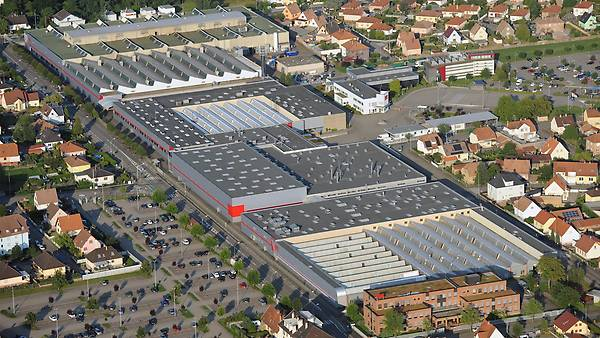
\includegraphics[scale=1,width=0.9\textwidth]{sew_haguenau.jpg}
    \caption{Vue de l'usine de Haguenau}%
    \label{fig:sew_haguenau}
  \end{figure}
\end{minipage}
\end{frame}
%
% %%%% --4--%%%%
\subsection{Etat actuel}
\begin{frame}
  \frametitle{Etat actuel}

  Gestion des stocks inexistantes entre les zones de production et de
  stockage et les autres usines.

  \textbf{Probl{\'e}matique~:} Avoir constamment des contenants vides sur
  les zones de production et suffisamment de contenants utiles {\`a} la
  production sur chaque site

  \begin{minipage}{.5\textwidth}
    \begin{figure}
      \centering
      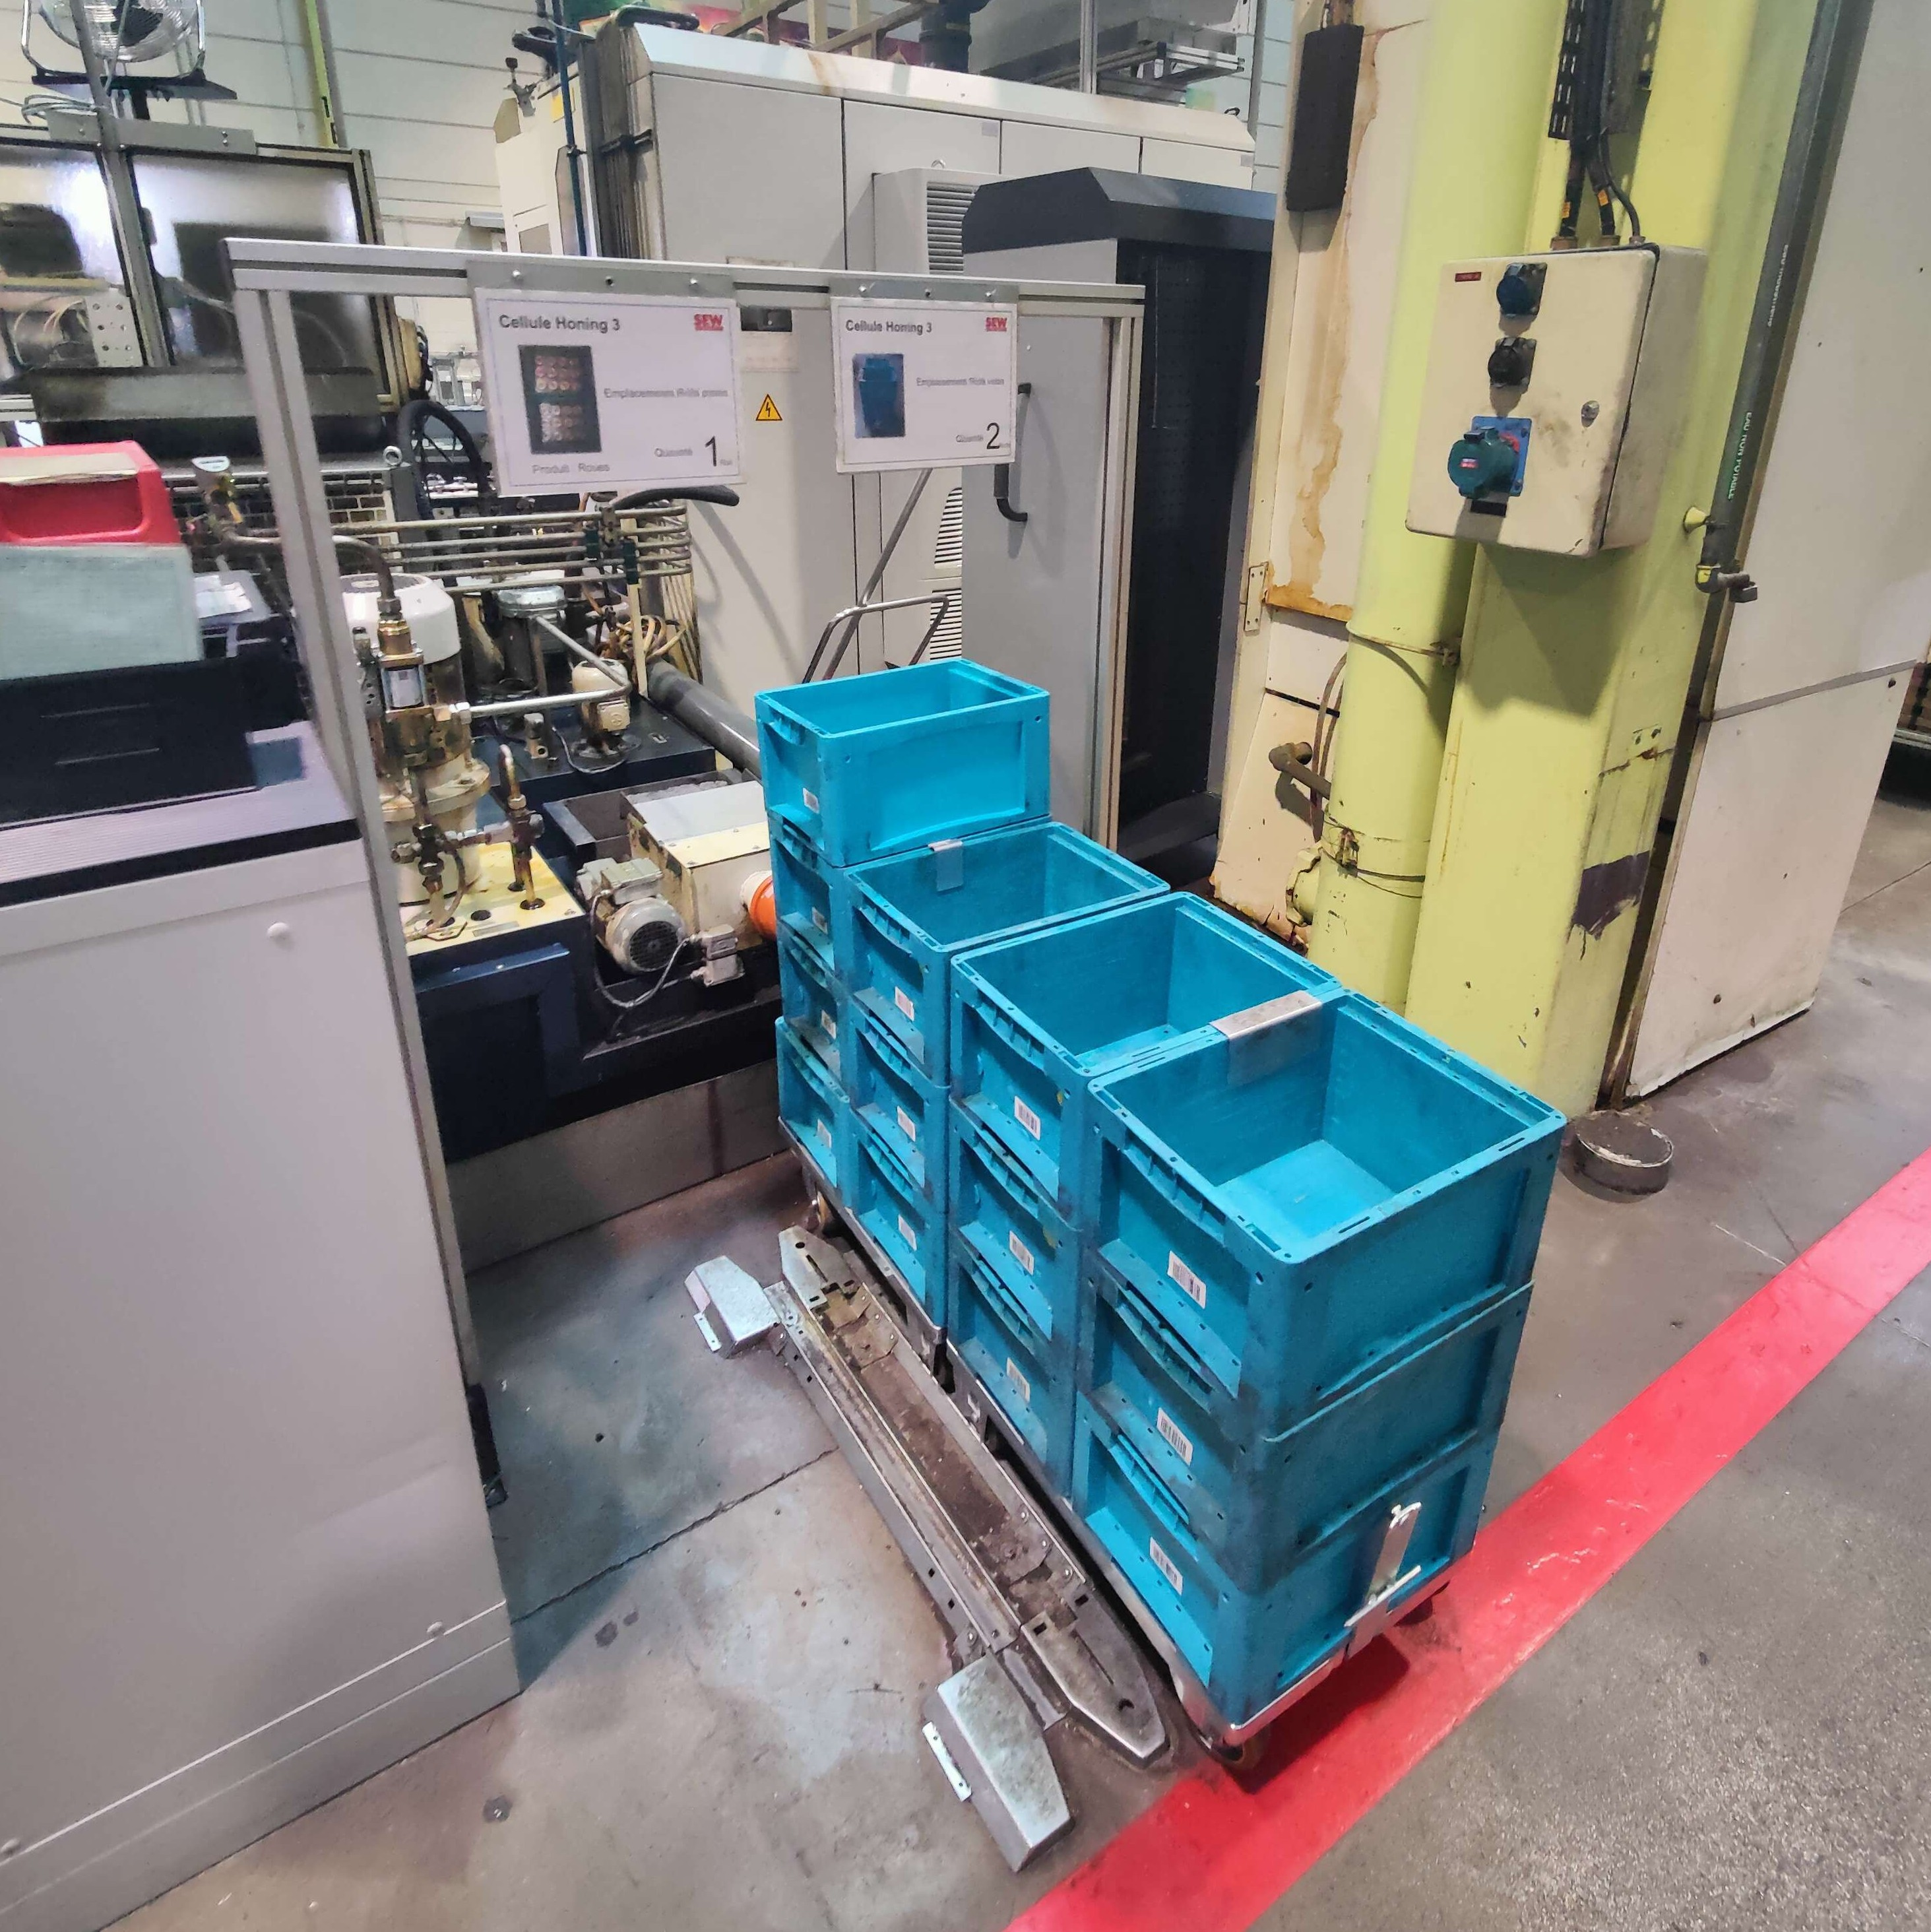
\includegraphics[width=0.7\textwidth, height=0.47\textheight]{sew_production.jpg}
      \caption{Image d'une zone de production d'Haguenau}%
      \label{fig:sew_production}
    \end{figure}
  \end{minipage}%
  \begin{minipage}{.5\textwidth}
    \begin{figure}
      \centering
      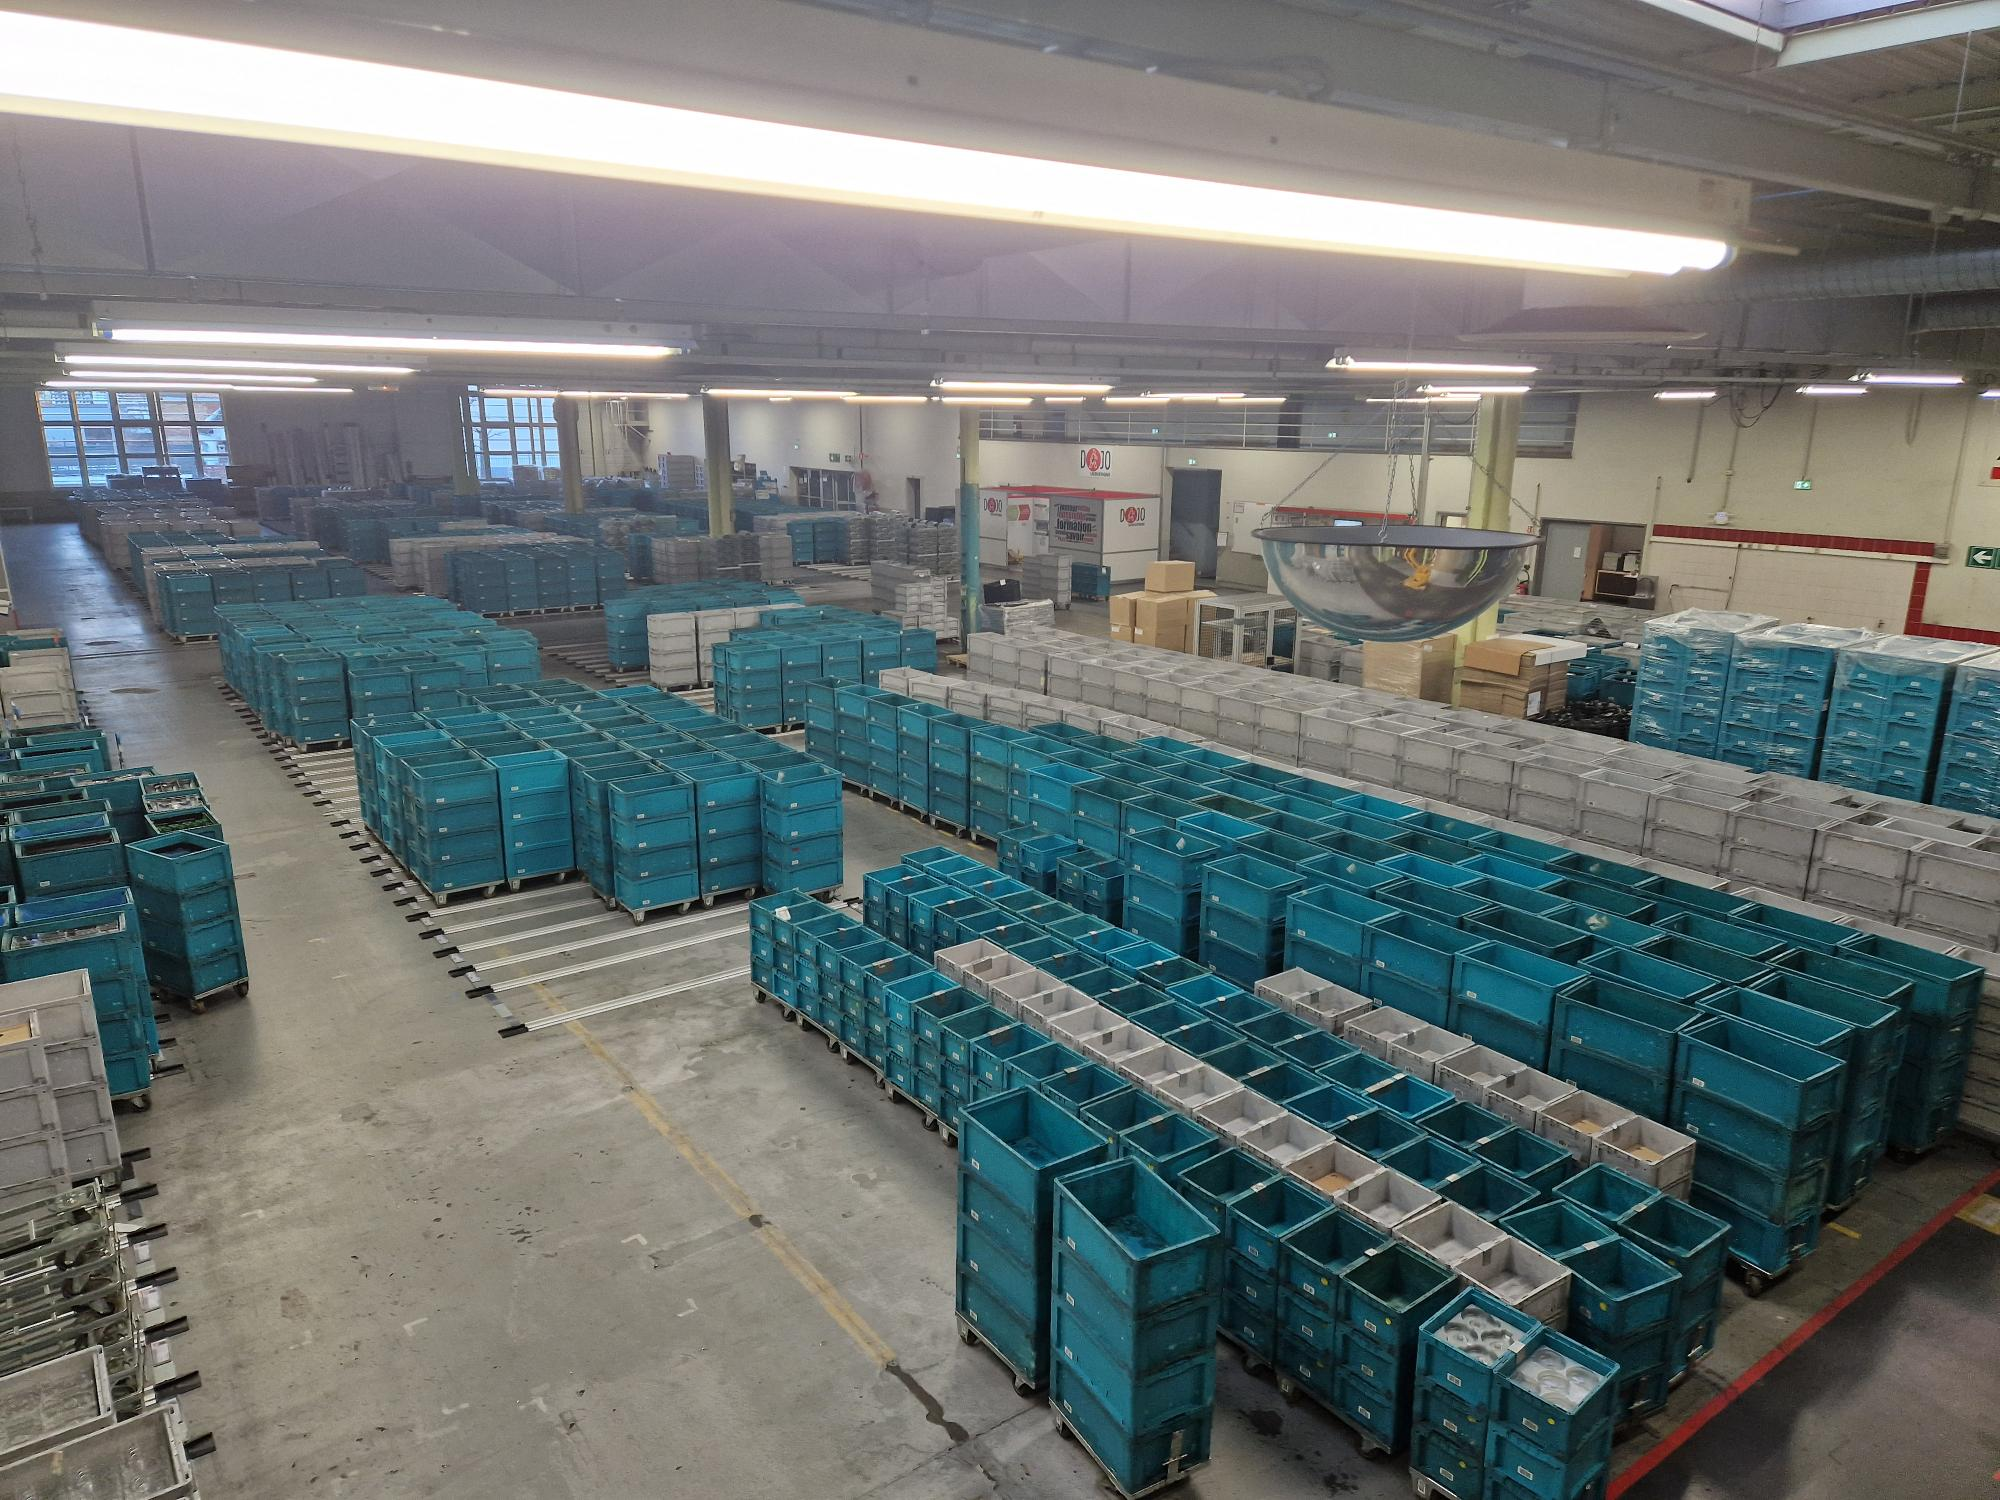
\includegraphics[scale=1,width=0.9\textwidth]{sew_entrepot.jpg}
      \caption{Image de la zone de stockage de Haguenau}%
      \label{fig:sew_entrepot}
    \end{figure}
  \end{minipage}
\end{frame}%
% %%% --5--%%%
\subsection{Objectifs du projet}
\begin{frame}
  \frametitle{Objectifs du projet}
  \textbf{Objectif principal~:} Classification et comptage des
  contenants vides

  \begin{center}
    \scriptsize
    \begin{tabular}{|p{3cm}|p{4.5cm}|p{3cm}|}
      \hline
      Objectifs & Crit{\`e}res & Moyens \\
      \hline
      Acquisition de donn{\'e}es num{\'e}riques & 1. Avoir assez d'images des
                                                  diff{\'e}rentes bo{\^\i}tes
                                                  r{\'e}parties
                                                  homog{\`e}nement &
                                                                     Utilisation de cam{\'e}ras IP \\
                & 2. Acquisition dans nos locaux et {\`a} SEW & \\
      \hline
      Classification des types de bo{\^\i}tes par apprentissage automatique &
                                                                              Classification
                                                                              des images avec
                                                                              environ
                                                                              90 \% de pr{\'e}cision & Utiliser Python et YOLO \\
      \hline
      Classification des bo{\^\i}tes vides ou non par apprentissage automatique
                & D{\'e}terminer si les bo{\^\i}tes sont vides ou non avec une
                  pr{\'e}cision tout autant {\'e}lev{\'e}e 90 \% & Utiliser Python
                                                                   et YOLO\\
      \hline
      Compter le nombre de bo{\^\i}tes & 1. Compter celles vides par types
                                         pr{\'e}c{\'e}demment identifi{\'e}es &\\
                & 2. Prendre en compte les bo{\^\i}tes cach{\'e}es &\\
      \hline
      Utilisation et explicabilit{\'e} du logiciel & 1. Rendre le logiciel
                                                     utilisable et compr{\'e}hensible & Installation
                                                                                        finale et contr{\^o}le du logiciel\\
                & 2. Possibilit{\'e} de changer les types de bo{\^\i}tes & \\ %rajout de bo{\^\i}tes par exemple
      \hline
    \end{tabular}
  \end{center}
\end{frame}
%%


% %%%% --4--%%%%
\section{Pr{\'e}vision des t{\^a}ches {\`a} r{\'e}aliser}
\subsection{Cahier des charges}
\begin{frame}
  \frametitle{Pr{\'e}vision des t{\^a}ches {\`a} r{\'e}aliser}
  \begin{itemize}
  \item Pr{\'e}sentation du cahier des charges + type de cam{\'e}ra envisag{\'e}
    donc budgets~?
  \item Diagramme de Gantt sur l'enti{\`e}ret{\'e} du projet
  \item Diagramme de Gantt pr{\'e}visionnel avant le R1 et diagramme effective
  \end{itemize}
\end{frame}
%
\subsection{Pr{\'e}vision des t{\^a}ches {\`a} r{\'e}aliser}
\begin{frame}
  \frametitle{Pr{\'e}vision des t{\^a}ches {\`a} r{\'e}aliser}
  \begin{figure}
    \centering
    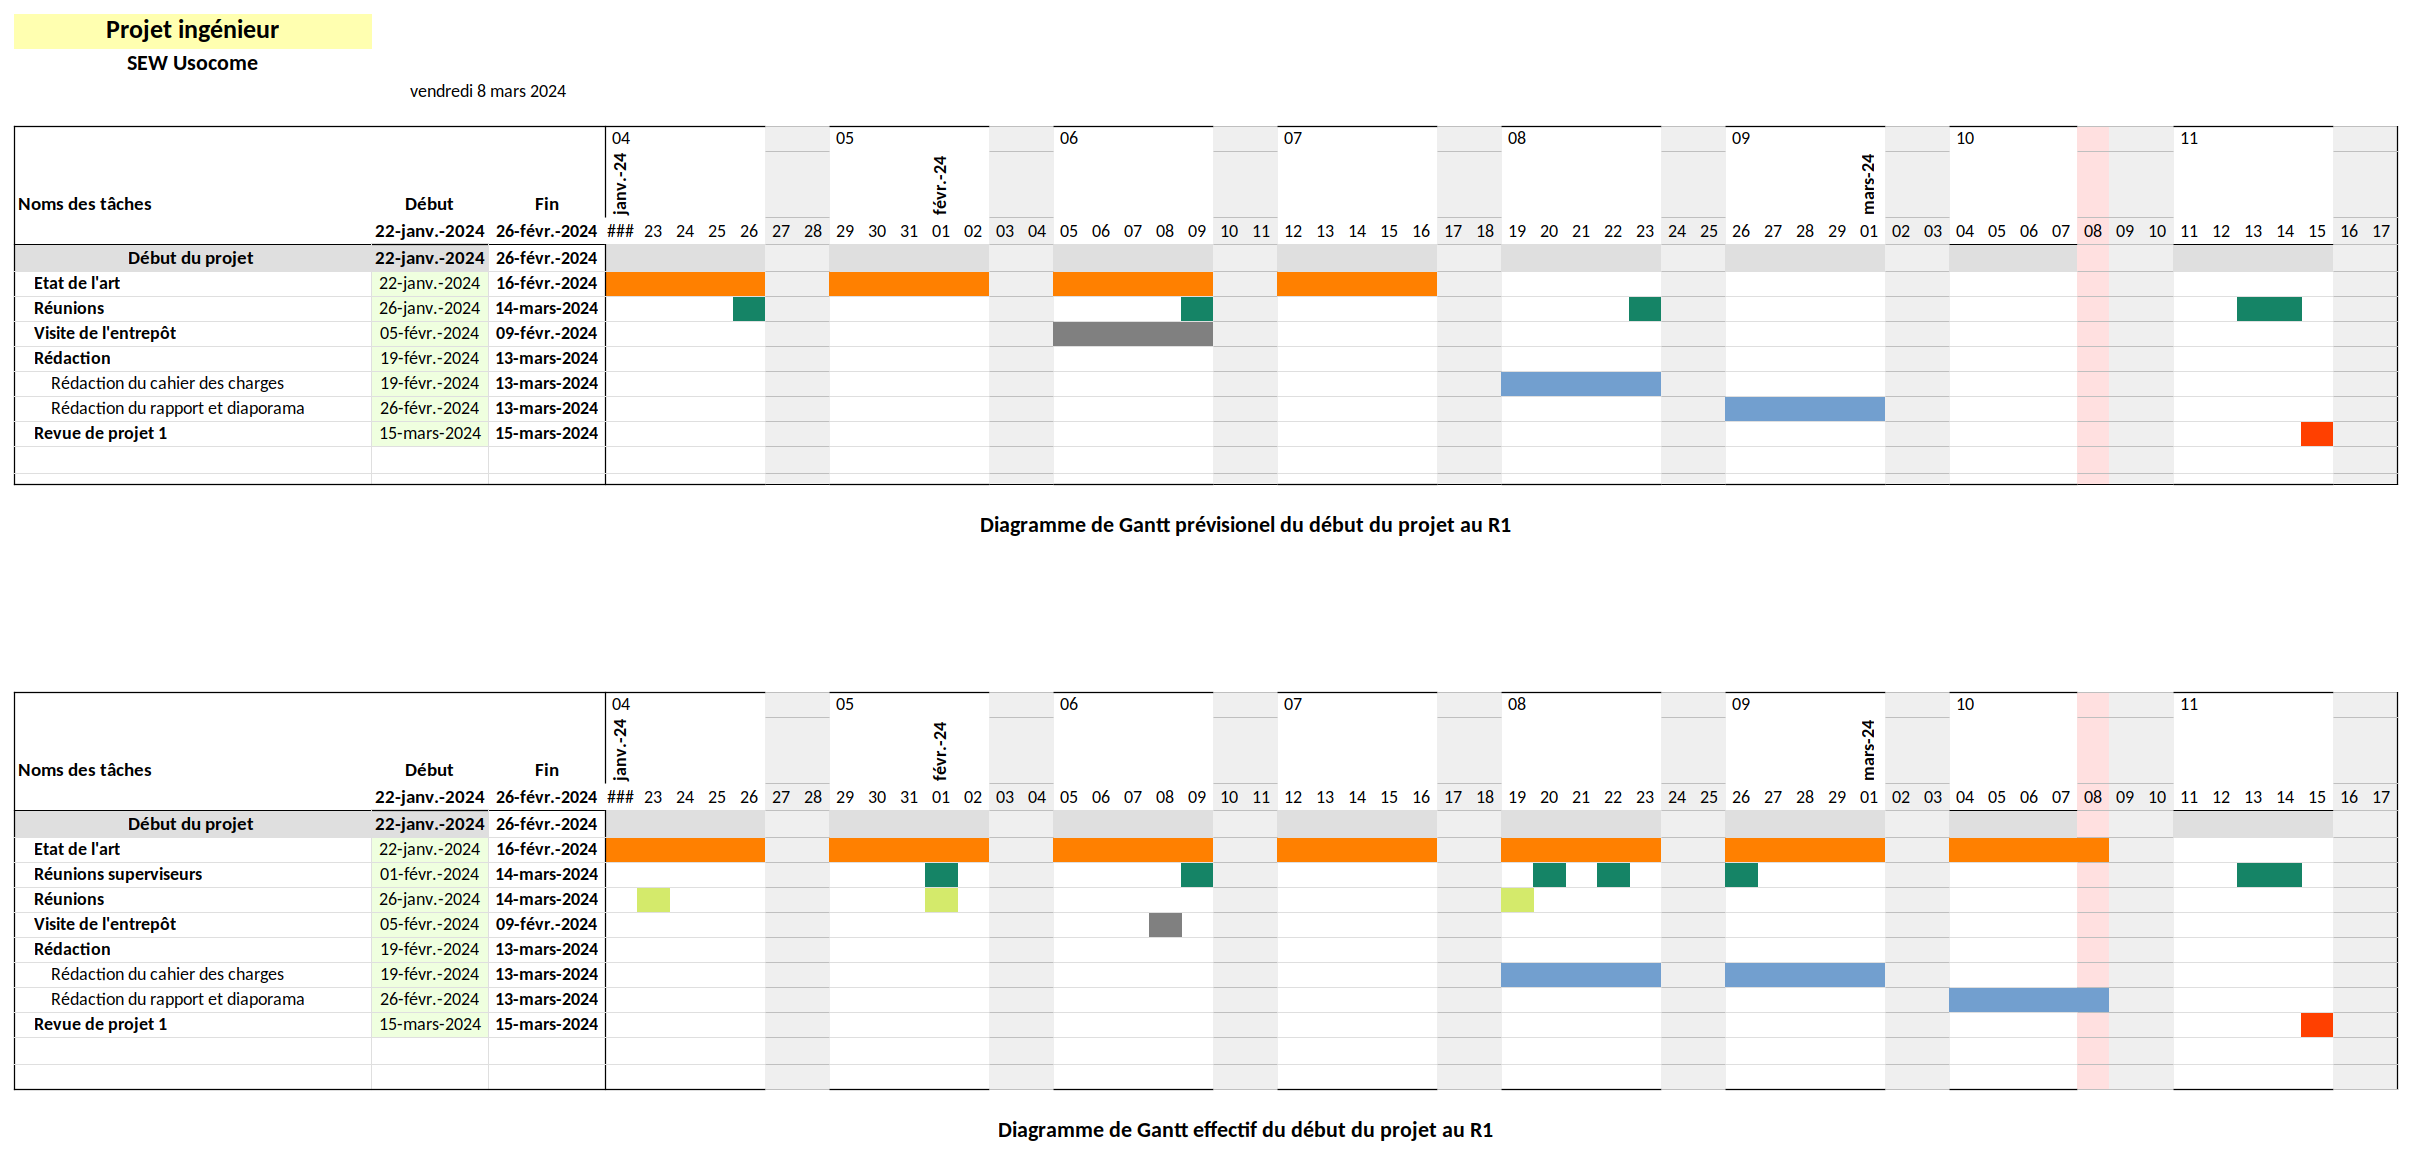
\includegraphics[width=0.9\textwidth, height=0.7\textheight]{gantt_r1.png}
    \caption{Diagramme de Gantt prévisionnel (en haut) et effectif (en
      bas) du projet avant la première revue}%
    \label{fig:gantt_r1}
  \end{figure}
\end{frame}
%
% %%%% --5--%%%%
\section{Etat de l'art}
\begin{frame}
  \frametitle{Remise en contexte}
  \begin{itemize}
  \item rfid (trop cher)
  \item vision (contours des bo{\^\i}tes)
  \item Plus important : YOLO mais d'autres existent mais moins
    utilis{\'e}s comme \textit{SDD ?}
  \end{itemize}
\end{frame}
%
% %%%% --6--%%%%
\section{Pistes de solutions}
\begin{frame}
  \frametitle{Pistes de solutions}
  \begin{itemize}
  \item Pour les zones de production~: comptage apr{\`e}s identification
    des bo{\^\i}tes vide ou non en ayant ou non d{\'e}finit quel type de bo{\^\i}te
  \item Pour la zone de stockage~: utilisation des zones strat{\'e}giques
    de passages pour une meilleure classification et s'affranchir des
    risques d'identification des bo{\^\i}tes cach{\'e}es
  \end{itemize}
\end{frame}
%
% %%%% --7--%%%%
%\section{Conclusion}
\begin{frame}
  \frametitle{Conclusion}
  Poursuite du PI~?
\end{frame}
% %%%% --7--%%%%
\begin{frame}
  \frametitle{Bibliographie}
  Pour print la biblio il faut utiliser les refs comme ceci
  \citeauthor{bib:ziou}. Pour actualiser la biblio~:
  \begin{itemize}
  \item pdflatex presentation\_R1.tex
  \item biber presentation\_R1
  \item pdflatex presentation\_R1.tex
  \end{itemize}

  \printbibliography%

  \begin{itemize}
  \item SEW usocome site \textit{usocome.com}
  \end{itemize}
\end{frame}
\end{document}
%
